\documentclass[12pt]{article}

\usepackage{amssymb,amsmath,amsthm}
\usepackage{graphicx}
\usepackage{fullpage}
\usepackage[final,colorlinks,hyperindex,unicode=true]{hyperref}
%\usepackage{tikz}
%\usepackage{pgfplots}
\usepackage[shadow,colorinlistoftodos,textwidth=3cm]{todonotes}
\usepackage{simplewick}

\usetikzlibrary{positioning,fadings,shapes,fit}

\def\myarc#1#2#3#4{
  \draw[color=#1,line width=2pt] (360*#2/18:#4mm) arc (360*#2/18:360*#3/18:#4mm);
}%#1 -- color, #2 -- from, #3 -- to, #4 -- radius (mm)

\begin{document}
\thispagestyle{empty}
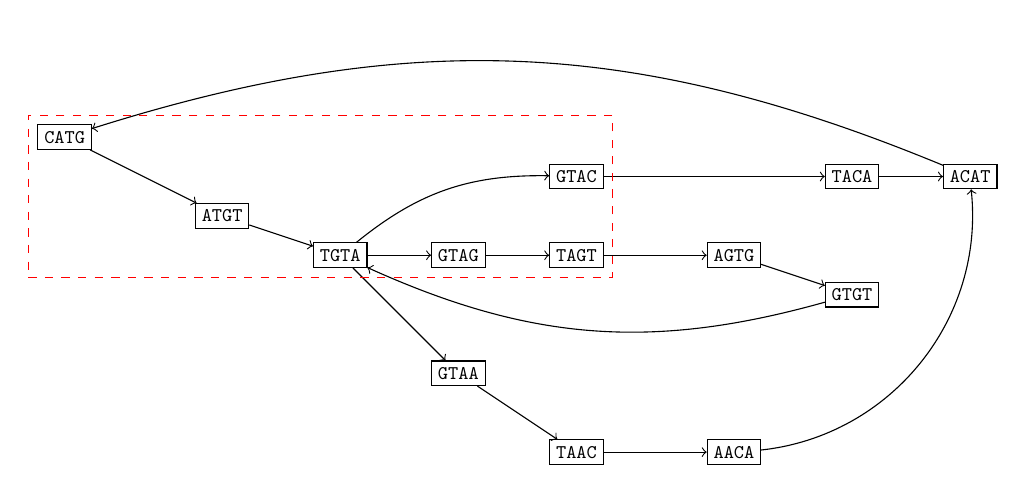
\begin{tikzpicture}
  %\node[anchor=south west] at (0,0) {\includegraphics[scale=0.4]{tmp.jpg}};
  %\draw[help lines,step=.5cm] (0,0) grid (20,10);
  %\foreach \x in {1,...,10} {
  %  \node at (-.5,\x) {\x};
  %  \node at (\x,-.5) {\x};
  %}

  \foreach \x/\y/\t in {0.5/4.5/CATG, 2.5/3.5/ATGT, 4/3/TGTA, 5.5/3/GTAG, 5.5/1.5/GTAA,
    7/4/GTAC, 7/3/TAGT, 7/0.5/TAAC, 9/3/AGTG, 9/0.5/AACA, 10.5/4/TACA, 10.5/2.5/GTGT, 12/4/ACAT}
  \node[draw,rectangle,scale=0.7] (\t) at (\x,\y) {{\tt \t}};

  \foreach \s/\t in {CATG/ATGT, ATGT/TGTA, TGTA/GTAG, GTAG/TAGT, 
  TAGT/AGTG, AGTG/GTGT, TGTA/GTAA, GTAA/TAAC, TAAC/AACA, GTAC/TACA, TACA/ACAT}
    \draw [->] (\s) to (\t);
  \draw [->] (GTGT) to[bend left=20] (TGTA);
  \draw [->] (TGTA) to[bend left=20] (GTAC);
  \draw [->] (AACA) to[bend right=45] (ACAT);
  \draw [->] (ACAT) to[bend right=20] (CATG);
  \node[rectangle,draw=red,dashed,fit=(CATG) (ATGT) (TGTA) (GTAG) (TAGT)] {};

\end{tikzpicture}
\end{document}
